\chapter{Results}
\label{ch:results}

The original MIT experiment is reported first, preserving its fixed comparisons. The chapter
then examines prediction and proxy response in the exploratory linear follow-up, followed by
the independent AVI-Personality prediction and group-error analysis. Their metric aggregation
and outcome scales are stated separately.

\section{Analysis sample and outcome measurement}

The verified corpus contains 69 participant pairs and 138 pre/post sessions with complete
audio, video, aggregate-rating and transcript joins. The canonical-to-source mapping corrects
the reciprocal post-session 32/33 source labels before participant grouping and analysis. All
69 pairs passed the common modality-eligibility rule, so each configuration and seed has 138
held-out predictions. The target is the aggregate \emph{RecommendHiring} rating on its documented
1--7 scale, interpreted as crowd-perceived hireability rather than a hiring outcome. Mapping and
representation checks are documented in Appendix~\ref{app:reproducibility}.

The outcome audit covers 138 EM aggregates and 1,240 individual ratings from nine workers. Two
sessions have eight individual ratings and 136 have nine. Ordinal Krippendorff alpha
~\cite{Krippendorff2011} for the individual \emph{RecommendHiring} ratings is 0.232, indicating
low agreement and a material construct limitation. The EM aggregates are nevertheless strongly
associated with unweighted session means (Pearson 0.981, Spearman 0.977; raw-scale MAE
0.116). Mean aggregate ratings are 4.821 in pre sessions and 5.070 in post sessions;
the raw difference of 0.249 is descriptive and must not be interpreted causally.

Numerical estimates in this chapter are rounded to three decimals for display, except that a
fourth decimal is retained when three decimals would obscure a near-zero nonzero value. All
comparisons and intervals were calculated from unrounded values.

\section{Perceived-attribute annotation coverage}

All 126 supplied rows map uniquely to known canonical sessions, with no duplicate session or
blank required value. The post wave supplies one annotation for every participant; the pre wave
is missing for 12 participants. The source appearance codes denote White (\texttt{W}), Black
(\texttt{B}), East Asian (\texttt{EA}), South Asian (\texttt{SA}), Southeast Asian
(\texttt{SEA}) and Middle Eastern or North African (\texttt{MENA}) appearance. The source code
\texttt{CD} means cannot determine and is treated as unknown rather than a group.
Table~\ref{tab:annotation-intake} reports the
phase-specific counts that determine reportability before predictions are audited.

\begin{table}[htbp]
\centering
\caption{Single-observer perceived-attribute counts by session phase. Codes retain the source
vocabulary; \texttt{CD} means cannot determine. The same participants contribute to both
phases only where a pre-session rating exists.}
\label{tab:annotation-intake}
\small
\begin{tabular}{llrr}
\toprule
Axis & Source code & Post count & Pre count \\
\midrule
Gender presentation & F & 43 & 36 \\
 & M & 26 & 21 \\
\addlinespace
Skin tone (1--5) & 1 & 20 & 5 \\
 & 2 & 27 & 28 \\
 & 3 & 15 & 16 \\
 & 4 & 2 & 5 \\
 & 5 & 5 & 3 \\
\addlinespace
Racialised appearance & W & 24 & 19 \\
 & EA & 16 & 11 \\
 & MENA & 11 & 9 \\
 & SA & 7 & 5 \\
 & B & 5 & 5 \\
 & SEA & 2 & 6 \\
 & CD & 4 & 2 \\
\bottomrule
\end{tabular}
\end{table}
\FloatBarrier

Under the fixed minimum of 10 unique participants, the primary post audit can estimate disparity
for both observed gender-presentation groups, skin-tone values 1--3, and appearance categories
\texttt{W}, \texttt{EA} and \texttt{MENA}. The pre sensitivity can report both gender groups,
skin-tone values 2--3, and appearance categories \texttt{W} and \texttt{EA}. All other categories
are counted but their disparity estimates are suppressed, never merged. Two further appearance
codebook categories have zero rows in both phases and no estimate. The appearance code
\texttt{CD} records an unknown value (four post and two pre rows), not an appearance category in
the W1 calculation. Skin tone remains ordinal 1--5 and is not binarised. The source age field is
retained for provenance but excluded from both Stages B and C.

Across the 57 complete pairs, gender presentation matches in every pair, racialised appearance
matches in 31, and skin tone matches exactly in 26; 54 skin-tone pairs differ by at most one scale
step. These comparisons mix presentation, recording and phase with observer consistency and do
not provide inter-rater reliability. The source contains no reproducible rater identity,
field-level confidence, collection-instruction record or blinding record, so none is claimed.

\section{Evaluation roster and model comparisons}

All 69 participants were eligible; none was excluded. The 21 learned model--seed
combinations each cover the same 138 held-out sessions; nine deterministic references were evaluated on
the same roster. Perceived-attribute annotations were not used to fit or select ordinary models.

\begin{table}[htbp]
\centering
\caption{Participant-grouped evaluation roster and fixed comparison set.}
\label{tab:stage-a-release}
\begin{tabular}{lr}
\toprule
Item & Verified value \\
\midrule
Eligible participants & 69 \\
Eligible sessions & 138 \\
Participant counts in folds 0--4 & 14/14/14/14/13 \\
Exclusions & 0 \\
Learned configurations & 7 \\
Fixed seeds & 3 \\
Learned model--seed combinations & 21 \\
Participant-grouped learned fits & 105 \\
Deterministic diagnostic floors & 9 \\
Held-out predictions per model and seed & 138 \\
Prediction sets, including reference models & 30 \\
Perceived-attribute labels used in ordinary fitting & 0 \\
\bottomrule
\end{tabular}
\end{table}
\FloatBarrier

The independent sample remains 69 participants represented by 138 sessions. The 2,898 learned
prediction entries across seven configurations and three seeds are repeated predictions over that
common roster, not additional independent observations.

\section{Deterministic diagnostic floors}

\begin{table}[htbp]
\centering
\caption{Pooled OOF utility of the deterministic diagnostic floors. Each metric is calculated once
from the concatenated held-out predictions from all five folds; fold metrics are not averaged.
Errors are shown in original 1--7-scale units; normalised errors are exactly one sixth of these
values.}
\label{tab:stage-a-floors}
\small
\begin{adjustbox}{max width=\textwidth}
\begin{tabular}{lrrrr}
\toprule
Configuration & SRCC & Pearson & MAE$_{1--7}$ & RMSE$_{1--7}$ \\
\midrule
Mean & -0.206 & -0.187 & 0.590 & 0.739 \\
Phase mean & 0.074 & 0.018 & 0.573 & 0.731 \\
Video ridge & 0.138 & 0.065 & 0.714 & 0.947 \\
Audio ridge & 0.406 & 0.461 & 0.586 & 0.721 \\
Text ridge & -0.020 & 0.029 & 0.737 & 0.888 \\
Video--audio ridge & 0.424 & 0.456 & 0.542 & 0.687 \\
Video--text ridge & 0.147 & 0.108 & 0.640 & 0.826 \\
Audio--text ridge & 0.397 & 0.443 & 0.554 & 0.687 \\
All-modality ridge & 0.418 & 0.451 & 0.535 & 0.674 \\
\bottomrule
\end{tabular}
\end{adjustbox}
\end{table}
\FloatBarrier

The video--audio ridge floor had the highest observed floor SRCC (0.424). The all-modality ridge
floor had the lowest observed original-scale MAE (0.535) and RMSE (0.674). These are
diagnostic reference points, not estimates of audited disparity or deployment validity.

\section{Learned-model utility}

\begin{table}[htbp]
\centering
\caption{Pooled OOF utility of the seven learned configurations. Each entry is the arithmetic mean
$\pm$ sample SD across fixed seeds 1, 11 and 21. Each seed metric is computed from all held-out
session rows before the seed summary is formed. Errors are in original 1--7-scale units.}
\label{tab:stage-a-learned}
\small
\begin{adjustbox}{max width=\textwidth}
\begin{tabular}{lrrrr}
\toprule
Configuration & SRCC & Pearson & MAE$_{1--7}$ & RMSE$_{1--7}$ \\
\midrule
ERM & $0.170\pm0.123$ & $0.167\pm0.113$ & $0.951\pm0.227$ & $1.187\pm0.285$ \\
Face sampling & $0.192\pm0.124$ & $0.191\pm0.120$ & $0.915\pm0.118$ & $1.132\pm0.154$ \\
Audio sampling & $0.160\pm0.149$ & $0.168\pm0.133$ & $0.865\pm0.119$ & $1.077\pm0.149$ \\
Random-proxy W1 & $0.196\pm0.097$ & $0.195\pm0.098$ & $0.933\pm0.217$ & $1.159\pm0.263$ \\
Face-proxy W1 & $0.154\pm0.121$ & $0.151\pm0.109$ & $0.956\pm0.202$ & $1.198\pm0.256$ \\
Audio-proxy W1 & $0.113\pm0.149$ & $0.118\pm0.125$ & $0.894\pm0.144$ & $1.107\pm0.171$ \\
ARL & $0.157\pm0.135$ & $0.158\pm0.122$ & $0.946\pm0.230$ & $1.181\pm0.287$ \\
\bottomrule
\end{tabular}
\end{adjustbox}
\end{table}
\FloatBarrier

Across the seven learned configurations, mean SRCC ranged from 0.113 to 0.196 and mean
original-scale MAE ranged from 0.865 to 0.956. Random-proxy W1 had the highest observed
learned mean SRCC (0.196), while audio sampling alone had the lowest observed learned mean
original-scale MAE (0.865). Relative to its matched sampling-only counterpart, face W1 changed
mean SRCC by $-0.038$ and increased original-scale mean MAE by 0.040; audio W1 changed mean
SRCC by $-0.047$ and increased original-scale mean MAE by 0.029. Thus neither W1
configuration improved these two utility summaries over its corresponding sampling-only control.
This is a utility-only observation: it says nothing about whether either configuration changed
audited disparity. Seed-specific values appear in Appendix~\ref{tab:stage-a-seeds}.

For each of the four distinct utility metrics---SRCC, Pearson, MAE and RMSE---the best relevant
deterministic floor outperformed every learned three-seed mean and single-seed result. Reporting
MAE and RMSE on both the normalised and original rating scales does not create additional
independent metrics. For example, the best floor SRCC was
0.424, compared with 0.327 for the best learned single-seed result and 0.196 for the best
learned mean. The lowest floor original-scale MAE was 0.535, compared with 0.700 for the
best learned single-seed result and 0.865 for the best learned mean. The random-proxy control
also increased mean SRCC by 0.026 and reduced mean original-scale MAE by 0.017 relative to
ERM. This descriptive result prevents attributing a utility difference specifically to meaningful
visual or audio proxy structure.

For every learned configuration, seed 21 produced the highest SRCC and Pearson correlation and the
lowest MAE and RMSE on either rating scale. This systematic pattern, together with the
sample SDs, demonstrates material optimisation sensitivity; the three fixed seeds are not confidence
intervals, standard errors or evidence that one learned configuration is generally superior.
Likewise, Stage A contains no protected-attribute annotations and cannot establish that a proxy,
sampling policy, W1 penalty or ARL reduced disparity.

\section{Participant-cluster uncertainty and fixed utility contrasts}

The predeclared secondary report was executed after the prediction release was locked. It used
10,000 percentile-bootstrap resamples of the 69 participants with seed 2026, retaining both
sessions and all same-seed predictions whenever a participant was sampled. These are pointwise,
descriptive 95\% intervals; they are not multiple-comparison-adjusted tests. The strongest floor,
video--audio ridge, retained a positive pooled association (SRCC 0.424, 95\% interval
[0.240, 0.580]; Pearson 0.456 [0.298, 0.591]). Its original-scale MAE was 0.542
[0.468, 0.622]. The learned three-seed summaries were weaker: ERM mean SRCC was 0.170
[0.025, 0.303], and random-proxy W1 mean SRCC was 0.196
[0.049, 0.327].

Table~\ref{tab:stage-a-utility-contrasts} reports the six predeclared same-seed configuration
contrasts. Correlation changes are intervention minus reference; positive error improvements are
reference minus intervention, so positive values favour the intervention. Each point estimate is
the arithmetic mean of the three fixed within-seed contrasts, and each interval recomputes that
mean inside every participant resample.

\begin{table}[htbp]
\centering
\caption{Post-lock secondary utility contrasts with pointwise participant-cluster 95\% percentile
intervals. MAE and RMSE improvements are in original 1--7-scale units.}
\label{tab:stage-a-utility-contrasts}
\small
\textit{Correlation changes}\par\smallskip
\begin{adjustbox}{max width=\textwidth}
\begin{tabular}{lcc}
\toprule
Contrast & SRCC change & Pearson change \\
\midrule
Visual W1 vs ERM & $-0.016$ [$-0.058$, 0.022] & $-0.016$ [$-0.056$, 0.020] \\
Audio W1 vs ERM & $-0.057$ [$-0.130$, 0.018] & $-0.049$ [$-0.122$, 0.023] \\
Visual W1 vs visual sampling & $-0.038$ [$-0.072$, $-0.005$] & $-0.040$ [$-0.075$, $-0.006$] \\
Audio W1 vs audio sampling & $-0.047$ [$-0.091$, $-0.002$] & $-0.050$ [$-0.090$, $-0.014$] \\
Random-proxy W1 vs ERM & 0.026 [$-0.044$, 0.092] & 0.029 [$-0.044$, 0.096] \\
ARL vs ERM & $-0.013$ [$-0.033$, 0.005] & $-0.009$ [$-0.026$, 0.006] \\
\bottomrule
\end{tabular}
\end{adjustbox}

\medskip
\textit{Original-scale error improvements}\par\smallskip
\begin{adjustbox}{max width=\textwidth}
\begin{tabular}{lcc}
\toprule
Contrast & MAE improvement & RMSE improvement \\
\midrule
Visual W1 vs ERM & $-0.005$ [$-0.035$, 0.024] & $-0.012$ [$-0.043$, 0.018] \\
Audio W1 vs ERM & 0.057 [$-0.005$, 0.121] & 0.080 [0.009, 0.155] \\
Visual W1 vs visual sampling & $-0.040$ [$-0.080$, $-0.004$] & $-0.067$ [$-0.115$, $-0.020$] \\
Audio W1 vs audio sampling & $-0.029$ [$-0.059$, $-0.0001$] & $-0.030$ [$-0.056$, $-0.005$] \\
Random-proxy W1 vs ERM & 0.017 [$-0.037$, 0.073] & 0.028 [$-0.038$, 0.101] \\
ARL vs ERM & 0.004 [$-0.012$, 0.023] & 0.006 [$-0.010$, 0.023] \\
\bottomrule
\end{tabular}
\end{adjustbox}
\end{table}
\FloatBarrier

The total visual-W1, total audio-W1, random-proxy and ARL correlation intervals all include zero.
The isolated positive audio-W1 RMSE interval relative to ERM is not accompanied by a resolved
correlation or MAE contrast. By contrast, both incremental W1 comparisons favour their matched
sampling-only references on all four displayed metrics: every interval is below zero. This
supports the narrow conclusion that, under the frozen architecture and penalty, adding W1 did not
improve predictive utility beyond the associated balanced sampler. It is not evidence about
audited disparity.

Phase-stratified learned utility was also weaker after coaching. For example, ERM mean SRCC was
0.259 [0.105, 0.393] before coaching and 0.084 [$-0.101$, 0.262] after coaching.
Every learned configuration's pre-session mean SRCC interval excluded zero, whereas every
post-session interval included zero. None of the learned paired-change SRCC intervals excluded
zero. ERM's mean signed change bias was $-0.271$ on the original scale
[$-0.472$, $-0.084$], meaning that its predicted pre--post change was smaller on average than
the observed rating change. These are descriptive tracking results and cannot identify a coaching
effect.

\section{Proxy stability and representation coverage}

Proxy assignments were seed-invariant within each fold. Visual proxy partitions were identical up to neutral
label permutation across all outer rotations (all pairwise adjusted Rand index, ARI, and normalised mutual information, NMI, equal
1.0). Interview-audio proxy stability was lower (pairwise ARI 0.628--1.0; NMI
0.539--1.0). These common-roster comparisons describe the partitions produced by different
training folds; they are not independent held-out classification estimates. Neutral cluster
numbers can reverse between folds. Concatenating their unaligned identifiers would therefore
not produce a meaningful pooled partition. The mechanism analysis below instead uses each
held-out fold's own fitted groups and reports the corresponding score distances separately.

All 138 sessions had usable summaries for the three modalities and non-empty candidate text.
Every session reached the 128-face sample cap, and 66 required temporal audio subsampling beyond
the 16-window cap. Thus the visual and interview-audio representations are bounded summaries,
not exhaustive records of each interview.

\section{Inference-only modality-mask diagnostics}

For each locked ERM fit, one training-standardised modality summary was set to zero at inference;
the model was not refitted, selected or retuned. Table~\ref{tab:stage-a-masks} gives the arithmetic
mean and sample SD across fixed seeds. Positive changes favour the masked prediction.

\begin{table}[htbp]
\centering
\caption{Inference-only modality-mask diagnostics on locked ERM predictions. Error improvements
are in original 1--7-scale units. Values are mean $\pm$ sample SD across three fixed seeds.}
\label{tab:stage-a-masks}
\small
\begin{adjustbox}{max width=\textwidth}
\begin{tabular}{lrrrr}
\toprule
Masked modality & Masked SRCC & SRCC change & MAE improvement & RMSE improvement \\
\midrule
Video & $0.230\pm0.060$ & $0.060\pm0.073$ & $0.155\pm0.148$ & $0.208\pm0.185$ \\
Interview audio & $-0.155\pm0.131$ & $-0.325\pm0.048$ & $0.042\pm0.072$ & $0.059\pm0.125$ \\
Candidate text & $0.253\pm0.026$ & $0.083\pm0.097$ & $0.157\pm0.273$ & $0.214\pm0.318$ \\
\bottomrule
\end{tabular}
\end{adjustbox}
\end{table}
\FloatBarrier

Masking interview audio reduced SRCC in every seed and produced the largest, most consistent rank
change. Masking video or candidate text sometimes improved aggregate error metrics. Within this
locked ERM implementation, rank predictions therefore depend strongly on the interview-audio
summary, while the video and text contributions appear less consistently useful. Because zero-mask
inference can move a model off its training distribution, this is a dependence diagnostic, not a
causal ablation, a modality-specific retraining comparison, a confidence interval or a fairness
result.

\section{Phase-aligned perceived-attribute audit}

The exploratory perceived-gender oracle produced 15 cross-fitted fits and 138 held-out
predictions per seed. It is included as a separately labelled, annotation-supervised comparison,
not as a protected-label-free method or performance ceiling. The primary audit compares each
model's post-session predictions with the 69 post-session annotations. A separate sensitivity
uses only the 57 participants with pre-session annotations. The participant-cluster intervals
resample phase-matched participants 10,000 times. Ordinary models, proxies and predictions
were fixed before annotations were joined for the audit.

\subsection{Primary post-session perceived-attribute disparity}

Table~\ref{tab:stage-c-disparity} reports the maximum pairwise empirical Wasserstein-1 distance
between \emph{predicted scores} for reportable
categories on each perceived-attribute axis. Scores use the normalised 0--1 target scale. Each
category requires at least ten distinct participants; the racialised-appearance and skin-tone
axes retain their original categories rather than being reduced to binary groups. For each
learned configuration, a cell shows the minimum and maximum of three separate seed-specific
distances. These ranges are descriptive seed sensitivity, \emph{not} confidence intervals or
seed-matched contrasts. The phase-matched post roster contains 69 participants, but the
reportable categories entering each pairwise distance contain 69 participants for gender
presentation, 51 for racialised appearance and 62 for skin tone. The remaining records are
unknown or belong to suppressed categories (Table~\ref{tab:annotation-intake}).

\begin{table}[htbp]
\centering
\caption[Post-session predicted-score disparity across perceived groups]{Post-session score disparity measured by maximum pairwise W1. Learned-model
cells are minimum--maximum across fixed seeds 1, 11 and 21, not bootstrap intervals;
deterministic-floor cells are single cross-fitted values. All values use the normalised 0--1 scale.}
\label{tab:stage-c-disparity}
\small
\smallskip
\begin{adjustbox}{max width=\textwidth}
\begin{tabular}{lccc}
\toprule
Configuration & Gender presentation & Racialised appearance & Skin tone \\
\midrule
\multicolumn{4}{l}{\textit{Learned configurations: three-seed minimum--maximum}} \\
ERM & 0.027--0.094 & 0.043--0.083 & 0.054--0.089 \\
Face sampling only & 0.038--0.059 & 0.044--0.071 & 0.046--0.098 \\
Interview-audio sampling only & 0.030--0.067 & 0.040--0.084 & 0.052--0.096 \\
Random-proxy W1 & 0.036--0.104 & 0.037--0.075 & 0.057--0.081 \\
Face-proxy W1 & 0.039--0.062 & 0.049--0.088 & 0.052--0.081 \\
Interview-audio-proxy W1 & 0.030--0.054 & 0.055--0.078 & 0.068--0.098 \\
ARL & 0.030--0.093 & 0.041--0.087 & 0.054--0.090 \\
Perceived-gender oracle & 0.048--0.057 & 0.052--0.072 & 0.056--0.109 \\
\midrule
\multicolumn{4}{l}{\textit{Deterministic floors: one cross-fitted value}} \\
Mean & 0.002 & 0.009 & 0.007 \\
Phase mean & 0.002 & 0.009 & 0.006 \\
Video ridge & 0.082 & 0.054 & 0.046 \\
Audio ridge & 0.054 & 0.061 & 0.068 \\
Text ridge & 0.027 & 0.072 & 0.054 \\
Video--audio ridge & 0.046 & 0.046 & 0.059 \\
Video--text ridge & 0.041 & 0.030 & 0.034 \\
Audio--text ridge & 0.049 & 0.038 & 0.069 \\
All-modality ridge & 0.049 & 0.030 & 0.066 \\
\bottomrule
\end{tabular}
\end{adjustbox}
\end{table}
\FloatBarrier

This table summarises all 99 reported configuration-by-axis values: 72 learned-model
seed-by-axis values and 27 fixed-floor values. The small predicted-score distances of the mean and
phase-mean floors illustrate why low disparity cannot be interpreted without utility: their
pooled SRCC values were $-0.206$ and 0.074, respectively
(Table~\ref{tab:stage-a-floors}). Neither these distances nor the learned-model seed ranges
establish whether a W1 penalty reduced audited disparity. The seed-matched comparisons below
address that narrower question.

\subsection{Observed-target disparity and reportability}

The observed crowd-perceived hireability target has nonzero empirical distances across the
reportable perceived groups
(Table~\ref{tab:stage-c-observed-target}). Each point is the largest pairwise empirical W1
distance among the reportable categories in that phase, with a pointwise participant-cluster
percentile interval. W1 is nonnegative, and an interval around the observed distance is not a
null test of equal population distributions. Thus a nonzero predicted-score distance is not
automatically a model-created disparity; nor does equality with the observed-target distance
validate a score.
The pre values describe a different, incompletely observed phase roster and are not direct
estimates of change from the post values.

\begin{table}[htbp]
\centering
\caption[Observed-target disparity by phase and perceived axis]{Observed-target maximum-pairwise W1 on the normalised 0--1 scale. Brackets are pointwise
95\% participant-cluster percentile intervals from 10,000 resamples. The attaining pair is the
pair at the point estimate; it may differ across resamples. Category abbreviations and counts
are given in Table~\ref{tab:annotation-intake}.}
\label{tab:stage-c-observed-target}
\small
\begin{adjustbox}{max width=\textwidth}
\begin{tabular}{lllc}
\toprule
Phase & Perceived axis & Attaining pair & Target W1 [95\% interval] \\
\midrule
Post ($n=69$) & Gender presentation & F--M & 0.046 [0.022, 0.104] \\
 & Racialised appearance & W--MENA & 0.052 [0.043, 0.125] \\
 & Skin tone & 1--2 & 0.070 [0.041, 0.133] \\
\midrule
Pre ($n=57$) & Gender presentation & F--M & 0.032 [0.027, 0.093] \\
 & Racialised appearance & W--EA & 0.038 [0.035, 0.108] \\
 & Skin tone & 2--3 & 0.040 [0.029, 0.110] \\
\bottomrule
\end{tabular}
\end{adjustbox}
\end{table}
\FloatBarrier

The post audit reports all 99 configuration-by-axis prediction summaries; the pre sensitivity
also reports 99. This does \emph{not} mean every source category is estimable.
The threshold is ten distinct participants per category. In the post wave, four appearance
labels are unknown; appearance B (5), SA (7) and SEA (2), skin-tone values 4 (2) and 5 (5),
and two unobserved appearance codebook categories are suppressed. In the pre wave, two
appearance labels are unknown; appearance B (5), SA (5), SEA (6) and MENA (9), skin-tone values
1 (5), 4 (5) and 5 (3), and the same two unobserved categories are suppressed. Gender
presentation has no unknown or suppressed observed category in either phase. Suppressed
categories are counted but never merged or assigned a subgroup disparity estimate.
All 10,000 replicates were valid for each reported three-seed disparity contrast in both phases.

\subsection{Seed-matched post-session disparity contrasts}

The two predeclared total-effect contrasts compare visual-proxy W1 and interview-audio-proxy W1
separately with the same-seed ERM reference. A positive disparity \emph{gain} means the reference
had greater maximum-pairwise predicted-score W1 than the intervention; a negative gain means
the intervention had greater W1. For each axis, the point estimate is the arithmetic mean of
the three seed-matched gains. Each interval recomputes the three-seed mean within every
69-participant bootstrap resample. Table~\ref{tab:stage-c-disparity-contrasts} retains the
seed-specific results rather than treating the three seeds as independent participants.

\begin{table}[htbp]
\centering
\caption{Primary post-session, same-seed disparity gains (ERM minus each W1 configuration)
on the normalised 0--1 scale. Mean is the three-seed arithmetic mean; brackets give the
pointwise 95\% participant-cluster interval. Positive values denote lower predicted-score
disparity under W1.}
\label{tab:stage-c-disparity-contrasts}
\small
\begin{adjustbox}{max width=\textwidth}
\begin{tabular}{lrrrrl}
\toprule
Perceived axis & Seed 1 & Seed 11 & Seed 21 & Mean & 95\% interval \\
\midrule
\multicolumn{6}{l}{\textit{Visual-proxy W1 versus ERM}} \\
Gender presentation & $-0.012$ & 0.032 & 0.006 & 0.009 & [$-0.009$, 0.024] \\
Racialised appearance & 0.006 & $-0.006$ & $-0.005$ & $-0.002$ & [$-0.017$, 0.015] \\
Skin tone & $-0.017$ & 0.003 & 0.008 & $-0.002$ & [$-0.021$, 0.015] \\
\midrule
\multicolumn{6}{l}{\textit{Interview-audio-proxy W1 versus ERM}} \\
Gender presentation & $-0.003$ & 0.061 & 0.011 & 0.023 & [$-0.005$, 0.049] \\
Racialised appearance & $-0.012$ & 0.015 & $-0.012$ & $-0.003$ & [$-0.020$, 0.037] \\
Skin tone & $-0.016$ & $-0.013$ & $-0.009$ & $-0.013$ & [$-0.029$, 0.030] \\
\bottomrule
\end{tabular}
\end{adjustbox}
\end{table}

\begin{figure}[H]
\centering
% Each row: /contrasts three_seed_arithmetic_mean audited_disparity gain.normalized;
% interval: /participant_cluster_bootstrap/contrasts with key
% [contrast_id, "three_seed_mean", "disparity_gain:" + field], percentile_95.normalized.
% Rounded to six decimals for display; the immutable JSON retains full precision.
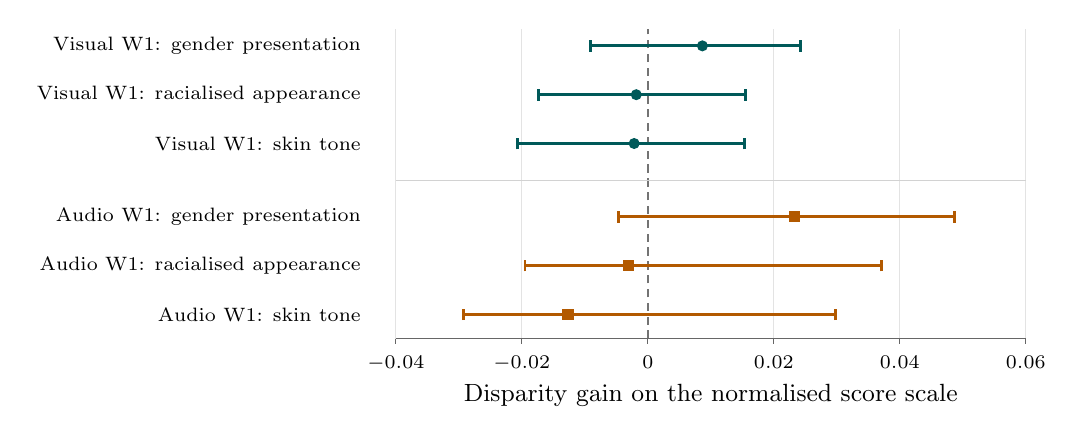
\begin{tikzpicture}[x=80cm,y=0.62cm]
  \foreach \x in {-0.04,-0.02,0.02,0.04,0.06} {
    \draw[gray!22] (\x,0.0) -- (\x,6.35);
  }
  \draw[black!55,densely dashed,line width=0.8pt] (0,0.0) -- (0,6.35);
  \draw[black!60] (-0.04,0.0) -- (0.06,0.0);
  \draw[gray!35] (-0.04,3.25) -- (0.06,3.25);

  \foreach \x/\label in {-0.04/$-0.04$,-0.02/$-0.02$,0/$0$,0.02/$0.02$,0.04/$0.04$,0.06/$0.06$} {
    \draw[black!60] (\x,0.0) -- (\x,-0.10);
    \node[font=\scriptsize,anchor=north] at (\x,-0.16) {\label};
  }
  \node[font=\small,anchor=north] at (0.01,-0.72)
    {Disparity gain on the normalised score scale};

  \node[font=\scriptsize,anchor=east] at (-0.044,6) {Visual W1: gender presentation};
  \node[font=\scriptsize,anchor=east] at (-0.044,5) {Visual W1: racialised appearance};
  \node[font=\scriptsize,anchor=east] at (-0.044,4) {Visual W1: skin tone};
  \node[font=\scriptsize,anchor=east] at (-0.044,2.5) {Audio W1: gender presentation};
  \node[font=\scriptsize,anchor=east] at (-0.044,1.5) {Audio W1: racialised appearance};
  \node[font=\scriptsize,anchor=east] at (-0.044,0.5) {Audio W1: skin tone};

  % Visual W1 versus same-seed ERM: pointwise 95% participant-cluster intervals.
  \draw[teal!70!black,line width=1pt] (-0.009153,6) -- (0.024242,6);
  \draw[teal!70!black,line width=1pt] (-0.009153,5.88) -- (-0.009153,6.12);
  \draw[teal!70!black,line width=1pt] (0.024242,5.88) -- (0.024242,6.12);
  \fill[teal!70!black] (0.008671,6) circle[radius=2pt];

  \draw[teal!70!black,line width=1pt] (-0.017332,5) -- (0.015458,5);
  \draw[teal!70!black,line width=1pt] (-0.017332,4.88) -- (-0.017332,5.12);
  \draw[teal!70!black,line width=1pt] (0.015458,4.88) -- (0.015458,5.12);
  \fill[teal!70!black] (-0.001826,5) circle[radius=2pt];

  \draw[teal!70!black,line width=1pt] (-0.020646,4) -- (0.015386,4);
  \draw[teal!70!black,line width=1pt] (-0.020646,3.88) -- (-0.020646,4.12);
  \draw[teal!70!black,line width=1pt] (0.015386,3.88) -- (0.015386,4.12);
  \fill[teal!70!black] (-0.002168,4) circle[radius=2pt];

  % Interview-audio W1 versus same-seed ERM, plotted with square markers.
  \draw[orange!70!black,line width=1pt] (-0.004588,2.5) -- (0.048720,2.5);
  \draw[orange!70!black,line width=1pt] (-0.004588,2.38) -- (-0.004588,2.62);
  \draw[orange!70!black,line width=1pt] (0.048720,2.38) -- (0.048720,2.62);
  \node[rectangle,fill=orange!70!black,minimum size=4pt,inner sep=0pt] at (0.023337,2.5) {};

  \draw[orange!70!black,line width=1pt] (-0.019508,1.5) -- (0.037087,1.5);
  \draw[orange!70!black,line width=1pt] (-0.019508,1.38) -- (-0.019508,1.62);
  \draw[orange!70!black,line width=1pt] (0.037087,1.38) -- (0.037087,1.62);
  \node[rectangle,fill=orange!70!black,minimum size=4pt,inner sep=0pt] at (-0.003113,1.5) {};

  \draw[orange!70!black,line width=1pt] (-0.029259,0.5) -- (0.029783,0.5);
  \draw[orange!70!black,line width=1pt] (-0.029259,0.38) -- (-0.029259,0.62);
  \draw[orange!70!black,line width=1pt] (0.029783,0.38) -- (0.029783,0.62);
  \node[rectangle,fill=orange!70!black,minimum size=4pt,inner sep=0pt] at (-0.012670,0.5) {};
\end{tikzpicture}

\caption{The six primary post-session three-seed mean disparity gains and pointwise 95\%
participant-cluster intervals from Table~\ref{tab:stage-c-disparity-contrasts}. The zero line
denotes no difference between each W1 configuration and same-seed ERM; positive values indicate
smaller predicted-score disparity under W1. These are perceived-attribute audit results, not
demographic-identity or hiring-fairness effects.}
\label{fig:stage-c-primary-disparity}
\end{figure}
\FloatBarrier

All six primary intervals cross zero (Figure~\ref{fig:stage-c-primary-disparity}); some
seed-specific gains also change sign. The data therefore do not resolve a reduction in any of
the three audited disparities for either W1 configuration relative to ERM. The intervals are
pointwise descriptive intervals over a fixed contrast family, without multiple-comparison
adjustment or automatic superiority tests.

Table~\ref{tab:stage-c-secondary-contrasts} gives the corresponding exploratory component and
control comparisons. Neither incremental W1 comparison with its matched sampling-only
configuration, the random-proxy comparison, ARL nor the protected-annotation oracle has a
three-seed mean disparity-gain interval excluding zero on any axis. The oracle was trained only
on the observed binary post-session perceived-gender-presentation field; it is neither a
protected-group-free method nor a performance upper bound. Its pooled original-scale MAE
improvement over ERM was $-0.068$ [$-0.108$, $-0.031$], while its pooled SRCC
change was $-0.010$ [$-0.057$, 0.032]. These contrasts do not support a
disparity--utility benefit for the oracle.

\begin{table}[htbp]
\centering
\caption{Secondary post-session three-seed mean disparity gains with pointwise 95\%
participant-cluster intervals, on the normalised 0--1 scale. Positive values denote lower
audited predicted-score W1 under the first configuration. Sampling comparisons isolate the
incremental W1 term; the remaining rows are
controls or an exploratory supervised oracle.}
\label{tab:stage-c-secondary-contrasts}
\small
\begin{adjustbox}{max width=\textwidth}
\begin{tabular}{lccc}
\toprule
Contrast & Gender presentation & Racialised appearance & Skin tone \\
\midrule
Visual W1 vs visual sampling & \shortstack{$-0.002$\\{[$-0.016$, 0.009]}} & \shortstack{$-0.006$\\{[$-0.023$, 0.012]}} & \shortstack{0.003\\{[$-0.017$, 0.017]}} \\
Audio W1 vs audio sampling & \shortstack{0.009\\{[$-0.006$, 0.022]}} & \shortstack{$-0.002$\\{[$-0.028$, 0.028]}} & \shortstack{$-0.006$\\{[$-0.022$, 0.017]}} \\
Random-proxy W1 vs ERM & \shortstack{$-0.007$\\{[$-0.029$, 0.020]}} & \shortstack{0.002\\{[$-0.027$, 0.029]}} & \shortstack{$-0.005$\\{[$-0.023$, 0.026]}} \\
ARL vs ERM & \shortstack{$-0.002$\\{[$-0.009$, 0.006]}} & \shortstack{$-0.006$\\{[$-0.023$, 0.016]}} & \shortstack{$-0.0003$\\{[$-0.013$, 0.012]}} \\
Perceived-gender oracle vs ERM & \shortstack{0.010\\{[$-0.016$, 0.032]}} & \shortstack{0.001\\{[$-0.028$, 0.018]}} & \shortstack{$-0.013$\\{[$-0.035$, 0.016]}} \\
\bottomrule
\end{tabular}
\end{adjustbox}
\end{table}
\FloatBarrier

\subsection{Proxy-to-perception association after prediction lock}

% Source: results/proxy-association-correction-2026-11-06.json.
The visual partition agrees exactly with the observer's post-session gender-presentation
codes in each outer test fold: NMI and ARI are both 1.000. The fold sizes are 14, 14, 14,
14 and 13 participants. A pooled description is possible only after resolving the
arbitrary cluster IDs. Alignment uses agreement among shared training participants,
without annotations or outcomes; it reveals the same visual partition up to a label
swap in every rotation. The aligned held-out groups contain 43 and 26 people and
retain NMI and ARI of 1.000 against this observer's gender-presentation codes.
Association with racialised appearance is much smaller (NMI 0.025, ARI 0.017;
65 known annotations), as is association with ordinal skin tone (NMI 0.012,
ARI $-0.003$; 69 annotations).

The audio partition changes beyond label swaps across rotations, so it does not support
a single pooled aligned group identity. Its fold-local held-out gender-presentation
NMI ranges from 0.002 to 0.094 and ARI from $-0.071$ to 0.026. These statistics describe
association with a single observer's perception of this corpus, not gender identity
or general demographic-classification accuracy. Perceived-group score disparities
above depend directly on annotations and are unaffected by cluster-number alignment.

\subsection{Annotation-conditioned errors}

Table~\ref{tab:stage-c-group-error} shows the reportable-category absolute errors and signed
residuals for ERM on the 69 post sessions. Each range is the minimum--maximum across fixed seeds
1, 11 and 21, \emph{not} a confidence interval. Errors are on the original 1--7 rating scale,
and residual is prediction minus target; a negative residual indicates underprediction of the
crowd rating. Categories on different axes overlap, so rows cannot be pooled as independent
subsamples. The aggregate also contains seed-specific group bootstrap intervals; this compact
table does not convert the ranges into a test of between-group error equality.

\begin{table}[htbp]
\centering
\caption{Post-session ERM error by reportable perceived category. Values are descriptive
minimum--maximum across the three fixed seeds on the original 1--7 rating scale; residual is
prediction minus crowd-perceived hireability.}
\label{tab:stage-c-group-error}
\small
\begin{adjustbox}{max width=\textwidth}
\begin{tabular}{llrrr}
\toprule
Perceived axis & Category & Participants & MAE range & Mean residual range \\
\midrule
Gender presentation & F & 43 & 0.755--1.223 & $-0.899$--$-0.240$ \\
 & M & 26 & 0.787--1.368 & $-1.161$--$-0.282$ \\
Racialised appearance & W & 24 & 0.997--1.308 & $-0.988$--$-0.431$ \\
 & EA & 16 & 0.680--1.288 & $-0.979$--$-0.112$ \\
 & MENA & 11 & 0.614--0.955 & $-0.558$--$-0.151$ \\
Skin tone & 1 & 20 & 0.880--1.316 & $-1.138$--$-0.601$ \\
 & 2 & 27 & 0.775--1.098 & $-0.762$--$-0.207$ \\
 & 3 & 15 & 0.562--1.262 & $-0.861$--0.079 \\
\bottomrule
\end{tabular}
\end{adjustbox}
\end{table}
\FloatBarrier

Absolute errors differ descriptively across these reported categories, but the same
seed-specific ranges often overlap and the small groups limit precision. Most listed ERM
residual ranges are negative. Neither pattern identifies bias against a verified demographic
group, and the suppressed categories have no error estimate.

\subsection{Pre-session sensitivity on available annotations}

The separate sensitivity uses only the 57 participants with pre-session annotations; the 12
missing pre annotations were neither imputed nor carried forward from post. This roster is not
assumed missing at random. The pre reportability pattern differs from the post pattern
(Table~\ref{tab:annotation-intake}): the reportable categories contain 57 participants for gender
presentation, 30 for racialised appearance and 44 for skin tone. Thus the maximum pairwise W1
can be attained by different category pairs. Table~\ref{tab:stage-c-pre-disparity-contrasts}
reports the same fixed contrast
family and sign convention, recomputed on the 57 pre sessions. All 21 three-seed mean pre
disparity-gain intervals cross zero. The pre results therefore do not rescue a mitigation claim
and do not estimate any causal pre/post or coaching effect.

\begin{table}[htbp]
\centering
\caption{Available-case pre-session three-seed mean disparity gains with pointwise 95\%
participant-cluster intervals ($n=57$), on the normalised 0--1 scale. Positive values denote lower
audited predicted-score W1 under the first configuration; category eligibility is recalculated
for the pre roster.}
\label{tab:stage-c-pre-disparity-contrasts}
\small
\begin{adjustbox}{max width=\textwidth}
\begin{tabular}{lccc}
\toprule
Contrast & Gender presentation & Racialised appearance & Skin tone \\
\midrule
Visual W1 vs ERM & \shortstack{0.010\\{[$-0.013$, 0.028]}} & \shortstack{$-0.005$\\{[$-0.025$, 0.018]}} & \shortstack{0.009\\{[$-0.014$, 0.027]}} \\
Audio W1 vs ERM & \shortstack{0.012\\{[$-0.010$, 0.032]}} & \shortstack{0.011\\{[$-0.015$, 0.033]}} & \shortstack{$-0.003$\\{[$-0.023$, 0.023]}} \\
Visual W1 vs visual sampling & \shortstack{0.001\\{[$-0.015$, 0.017]}} & \shortstack{0.002\\{[$-0.018$, 0.021]}} & \shortstack{0.013\\{[$-0.005$, 0.020]}} \\
Audio W1 vs audio sampling & \shortstack{0.005\\{[$-0.008$, 0.018]}} & \shortstack{0.011\\{[$-0.006$, 0.026]}} & \shortstack{0.003\\{[$-0.012$, 0.018]}} \\
Random-proxy W1 vs ERM & \shortstack{0.001\\{[$-0.022$, 0.021]}} & \shortstack{$-0.001$\\{[$-0.027$, 0.024]}} & \shortstack{$-0.002$\\{[$-0.022$, 0.019]}} \\
ARL vs ERM & \shortstack{$-0.002$\\{[$-0.009$, 0.008]}} & \shortstack{0.002\\{[$-0.011$, 0.012]}} & \shortstack{$-0.003$\\{[$-0.009$, 0.007]}} \\
Perceived-gender oracle vs ERM & \shortstack{0.013\\{[$-0.021$, 0.035]}} & \shortstack{$-0.011$\\{[$-0.032$, 0.020]}} & \shortstack{0.009\\{[$-0.019$, 0.028]}} \\
\bottomrule
\end{tabular}
\end{adjustbox}
\end{table}
\FloatBarrier

\subsection{Utility alongside audited disparity}

The six pooled-session utility contrasts and their participant-cluster intervals are reported in
Table~\ref{tab:stage-a-utility-contrasts}. They use both sessions of all 69 participants (138
held-out predictions per configuration and seed), whereas the primary perceived-attribute
disparity contrasts use one post session per participant. Reproducing pooled utility in Stage C
checks the same predictions rather than providing independent replication. For the post-only
roster, three-seed mean SRCC was 0.084 for ERM, 0.079 for visual W1 and 0.004 for
interview-audio W1; the corresponding original-scale MAEs were 1.025, 1.026 and 0.954.
These are descriptive phase-specific means, not a combined fairness--utility score or a
post-session interval comparison. The two incremental W1 contrasts had lower pooled correlation
and higher pooled errors than their matched sampling-only controls on all four utility measures.
The audio-W1 contrast with ERM had a positive pooled RMSE improvement but a negative, uncertain
SRCC change. Neither a general utility gain nor a simultaneous utility-and-disparity benefit is
supported by the fixed comparisons.

Every audited axis is a single-observer perception under the recorded video conditions, not
verified demographic identity. The source has no inter-rater agreement estimate and the
crowd-perceived target itself has low individual-rating agreement. The small category sizes,
pointwise intervals, incomplete pre wave and mixed-speaker interview audio further limit
generalisation. No result here establishes a causal coaching effect, hiring fairness,
employment-outcome validity or a legal-compliance judgement.

\section{Prediction with competitive linear scorers}
\label{sec:linear-results}

% Sources: results/study2_rq1_aggregate_v1.json; results/study2-compact-2026-10-21-aggregate.json.
The follow-up asks whether the weak original model obscured the behaviour of the penalty.
The natural-exposure linear reference reproduces the fixed all-modality ridge result:
pooled OOF SRCC 0.418 and normalised MAE 0.089 (original-scale MAE 0.535). It therefore
provides a materially stronger predictor than the original neural reference. This is not
evidence that linearity is universally preferable; it establishes a credible comparison
point for this small dataset and these frozen representations.

The separate outcome-only selection analysis chose tuned ridge in every outer rotation,
with alpha 1000 in all five. Table~\ref{tab:ridge-selection} reports the available outer-fold
summary. Its mean SRCC of 0.567 is an average of five within-fold correlations, while the
0.418 value above is calculated once from concatenated OOF predictions. These different
summaries must not be ranked as if their difference were a paired improvement estimate.
The selection summary supplies no uncertainty interval for that comparison.

\begin{table}[htbp]
\centering
\caption{Outcome-only predictive selection: unweighted means of five outer-fold metrics.
MAE uses the normalised MIT scale. These are not pooled OOF correlations.}
\label{tab:ridge-selection}
\begin{tabular}{lrr}
\toprule
Predictor & Mean fold MAE & Mean fold SRCC \\
\midrule
Phase-specific training mean & 0.096 & 0.226 \\
Selected tuned ridge & 0.081 & 0.567 \\
\bottomrule
\end{tabular}
\end{table}
\FloatBarrier

\section{Proxy response of the linear scorer}
\label{sec:compact-mechanism-results}

% Source: results/study2-compact-2026-10-21-aggregate.json.
The compact follow-up covers all 15 configurations and 75 outer-fold fits, yielding 2,070
held-out session predictions. Sixty-two fits meet their solver termination criterion.
Thirteen fits at the strongest coefficient, 0.2, reach the fixed iteration cap with finite
predictions. Every fit in the four primary strength-0.02 comparisons converged. The complete
grid in Table~\ref{tab:compact-grid} retains the capped results; those strongest-penalty
points describe bounded optimisation rather than established converged optima.

Unlike the original sampler comparison, the balanced-exposure control here evaluates the
full-fold group-weighted task objective. Its near-identical utility to natural exposure is
an observed result of this linear setting, not proof that balancing has no effect in other
models. Each W1 configuration changes only the penalty relative to its own exposure control.
All errors in the compact tables use the normalised MIT target scale.

\begin{table}[htbp]
\centering
\caption{Complete linear strength comparison on 138 pooled OOF sessions. All five test
folds are concatenated before each metric. A dagger identifies a configuration with at
least one iteration-capped fit; it is not a significance marker.}
\label{tab:compact-grid}
\small
\begin{tabular}{llrrr}
\toprule
Proxy & Task exposure & $\lambda$ & MAE & SRCC \\
\midrule
None & Natural & 0 & 0.089 & 0.418 \\
Visual & Balanced & 0 & 0.089 & 0.418 \\
Audio & Balanced & 0 & 0.089 & 0.418 \\
\addlinespace
Visual & Natural & 0.002 & 0.089 & 0.416 \\
 & & 0.02 & 0.090 & 0.389 \\
 & & $0.2^{\dagger}$ & 0.090 & 0.383 \\
Visual & Balanced & 0.002 & 0.089 & 0.416 \\
 & & 0.02 & 0.090 & 0.387 \\
 & & $0.2^{\dagger}$ & 0.089 & 0.392 \\
\addlinespace
Audio & Natural & 0.002 & 0.089 & 0.414 \\
 & & 0.02 & 0.091 & 0.374 \\
 & & $0.2^{\dagger}$ & 0.103 & 0.134 \\
Audio & Balanced & 0.002 & 0.089 & 0.414 \\
 & & 0.02 & 0.089 & 0.385 \\
 & & $0.2^{\dagger}$ & 0.103 & 0.129 \\
\bottomrule
\end{tabular}
\end{table}
\FloatBarrier

The penalty changes its intended quantity on both training and held-out proxy groups
(Table~\ref{tab:compact-manipulation}). For visual natural exposure at strength 0.02,
mean training W1 declines from 0.036 to 0.009 and mean held-out W1 from 0.045 to 0.035.
The audio natural-exposure comparison declines from 0.134 to 0.090 in training and from
0.087 to 0.068 on held-out groups. These distances are calculated within each fold's
own partition before the five distances are averaged. They establish an observed proxy
response rather than an audited-group fairness result.

\begin{table}[htbp]
\centering
\caption{Proxy manipulation at $\lambda=0.02$. Entries are arithmetic means of five
fold-specific W1 values. ``Control'' is the matched zero-penalty exposure.}
\label{tab:compact-manipulation}
\small
\begin{tabular}{llrrrr}
\toprule
Proxy & Exposure & Train control & Train W1 & Test control & Test W1 \\
\midrule
Visual & Natural & 0.036 & 0.009 & 0.045 & 0.035 \\
Visual & Balanced & 0.036 & 0.010 & 0.045 & 0.036 \\
Audio & Natural & 0.134 & 0.090 & 0.087 & 0.068 \\
Audio & Balanced & 0.134 & 0.096 & 0.087 & 0.070 \\
\bottomrule
\end{tabular}
\end{table}
\FloatBarrier

The response comes with a ranking cost. The visual natural-exposure SRCC change is
$-0.030$ with paired interval [$-0.069$, 0.008]. The audio natural-exposure change is
$-0.044$ [$-0.080$, $-0.008$]. Their normalised MAE changes are 0.001
[$-0.002$, 0.003] and 0.002 [$-0.001$, 0.005], respectively.
The balanced visual and audio SRCC changes are $-0.031$ [$-0.066$, 0.004] and
$-0.033$ [$-0.067$, 0.002]. These pointwise intervals condition on the fixed fitted
models; they do not include retraining or model-selection uncertainty. The strongest audio
coefficient also produces substantially lower point SRCC, but its capped optimisation
requires a separate numerical qualification.

\section{Transfer to perceived-group disparity}
\label{sec:compact-audit-results}

% Source: results/study2-compact-2026-10-21-aggregate.json.
The new phase-aligned audit uses the same single-observer source and reportable categories
as the original study. Its primary post roster remains 69 participants. On the working
natural-exposure reference, perceived-gender score W1 is 0.049. Visual W1 at strength 0.02
reduces the point estimate to 0.029, giving a gain of approximately 0.020. The paired
interval [$-0.005$, 0.025] includes zero, so the study does not resolve a population
reduction. The balanced visual comparison gives the same rounded gain with interval
[$-0.004$, 0.024].

Table~\ref{tab:compact-audit-gains} shows why the visual point change cannot be generalised
to every audited attribute. Racialised-appearance point gains are negative, while skin-tone
gains are small; every displayed interval crosses zero. The audio proxy also has a
smaller perceived-gender response than its own held-out proxy response would suggest.
Reducing the distance between two learned clusters therefore does not establish a
simultaneous improvement across the observer's other partitions.

\begin{table}[htbp]
\centering
\caption{Compact linear follow-up: primary post-session disparity gains at $\lambda=0.02$
relative to the exact exposure control. Positive values favour W1. Brackets are pointwise
95\% paired participant-percentile intervals; all values use the normalised score scale.}
\label{tab:compact-audit-gains}
\small
\begin{adjustbox}{max width=\textwidth}
\begin{tabular}{llccc}
\toprule
Proxy & Exposure & Gender presentation & Racialised appearance & Skin tone \\
\midrule
Visual & Natural & 0.020 [$-0.005$, 0.025] & $-0.009$ [$-0.015$, 0.010] & 0.001 [$-0.006$, 0.010] \\
Visual & Balanced & 0.020 [$-0.004$, 0.024] & $-0.007$ [$-0.013$, 0.010] & 0.001 [$-0.005$, 0.010] \\
Audio & Natural & 0.004 [$-0.002$, 0.011] & $-0.002$ [$-0.006$, 0.016] & 0.003 [$-0.002$, 0.013] \\
Audio & Balanced & 0.004 [$-0.002$, 0.010] & $-0.002$ [$-0.005$, 0.015] & 0.002 [$-0.003$, 0.012] \\
\bottomrule
\end{tabular}
\end{adjustbox}
\end{table}
\FloatBarrier

The separate 57-person pre sensitivity does not create a second observer or a replication.
Its visual perceived-gender gains are approximately 0.005, with intervals that include
zero. The audio gains are also about 0.005 and their lower interval endpoints round to
zero; this reduced, incompletely labelled phase cannot replace the primary post result.
All five ordinal skin-tone codes remain in the source counts and are not binarised.

Taken together, the linear results remove two ambiguities of the original experiment:
the comparison now uses a working predictor, and the penalty demonstrably changes the
observed proxy quantity on held-out participants. They do not remove the small-sample or
single-observer limits, and they do not establish a general disparity--utility improvement.

\section{AVI prediction and self-reported group error}
\label{sec:avi-results}

% Source: results/avi-baseline-2026-11-02-reconciled.json.
The AVI feature release covers 646 participants with six valid question clips each.
Supervised fitting uses 450 training participants; validation and test contain 64 and
130 participants. Ridge selection chooses alpha 1000, with validation MAE 0.415 on
the source 1--5 rating scale. On the official test, MAE is 0.419, compared with 0.479
for the training-target mean (Table~\ref{tab:avi-baseline}). The absolute improvement
is 0.060 rating points, approximately a 12.6\% reduction in MAE. This is a point
comparison on one held-out corpus, without a supplied paired uncertainty interval for
the utility improvement.

\begin{table}[htbp]
\centering
\caption[AVI-Personality baseline and descriptive group errors]{Independent AVI-Personality baseline on the original 1--5 interview-performance
scale. The official test contains 130 participants. Group results are descriptive.}
\label{tab:avi-baseline}
\begin{tabular}{lrr}
\toprule
Prediction or audit group & Test participants & MAE$_{1--5}$ \\
\midrule
Training-target mean reference & 130 & 0.479 \\
Validation-selected ridge & 130 & 0.419 \\
\addlinespace
Self-reported male & 67 & 0.452 \\
Self-reported female & 62 & 0.385 \\
Prefer not to say & 1 & Not estimated \\
Non-binary / third gender & 0 & Not estimated \\
\bottomrule
\end{tabular}
\end{table}
\FloatBarrier

The observed male-minus-female MAE difference is 0.067 rating points. It is a difference
in error against a recruiter rating, not in hiring outcomes or predicted-score parity.
The available absolute-gap bootstrap does not provide a signed-gap test, so the point
difference is not described as a statistically established population disparity. Sparse
and absent source categories remain visible and are not recoded to obtain an estimate.

This baseline supports the limited observation that the frozen video/audio
representations contain useful signal for a distinct interview rating. Taken on its own it
evaluates a predictive model and its group errors, without a penalised comparison; the
matched intervention and control arms reported in
Section~\ref{sec:avi-compact-results} are analysed separately below, after the baseline
and its audit had already been inspected. The raw AVI MAE is not ranked
against MIT MAE because the outcomes, scales and visual input boundaries differ.

\subsection{Matched proxy-penalty comparison on independent participants}
\label{sec:avi-compact-results}

% Source: results/avi-compact-reconciled-v1.json.
The fifteen fixed settings of Section~\ref{sec:avi-compact-method} were fitted on the same
feature release and evaluated on the official 130-participant test, giving 1{,}950 locked
prediction rows. Nine of the fifteen optimisations reported convergence; the remaining six
produced finite predictions but terminated without a convergence report. Those six are
retained in the complete grid and are described as bounded optimisation outcomes rather
than established optima. Table~\ref{tab:avi-compact-arms} gives the complete grid.

\begin{table}[htbp]
\centering
\caption[Complete AVI proxy-penalty grid]{Complete fifteen-arm grid on the independent
test. Errors are in original 1--5 rating units; score W1 is the Wasserstein-1 distance
between the predicted-score distributions of the two supported source gender groups, on the
normalised prediction scale. Prediction SD is reported against a target SD of 0.149.}
\label{tab:avi-compact-arms}
\small
\begin{adjustbox}{max width=\textwidth}
\begin{tabular}{llrrrrr}
\toprule
Proxy source & Exposure & $\lambda$ & MAE$_{1-5}$ & SRCC & Score W1 & Prediction SD \\
\midrule
None (control) & Natural & --- & 0.419 & 0.473 & 0.062 & 0.081 \\
\addlinespace
Visual & Natural & 0.002 & 0.419 & 0.473 & 0.061 & 0.081 \\
Visual & Natural & 0.02 & 0.421 & 0.455 & 0.061 & 0.080 \\
Visual & Natural & 0.2 & 0.424 & 0.445 & 0.059 & 0.078 \\
Audio & Natural & 0.002 & 0.419 & 0.473 & 0.061 & 0.081 \\
Audio & Natural & 0.02 & 0.422 & 0.442 & 0.057 & 0.074 \\
Audio & Natural & 0.2 & 0.453 & 0.295 & 0.050 & 0.067 \\
\addlinespace
Visual (control) & Balanced & --- & 0.420 & 0.463 & 0.064 & 0.083 \\
Visual & Balanced & 0.002 & 0.419 & 0.464 & 0.064 & 0.083 \\
Visual & Balanced & 0.02 & 0.417 & 0.464 & 0.065 & 0.083 \\
Visual & Balanced & 0.2 & 0.420 & 0.447 & 0.050 & 0.080 \\
\addlinespace
Audio (control) & Balanced & --- & 0.421 & 0.467 & 0.068 & 0.084 \\
Audio & Balanced & 0.002 & 0.421 & 0.466 & 0.068 & 0.083 \\
Audio & Balanced & 0.02 & 0.424 & 0.435 & 0.063 & 0.077 \\
Audio & Balanced & 0.2 & 0.462 & 0.320 & 0.054 & 0.070 \\
\bottomrule
\end{tabular}
\end{adjustbox}
\end{table}
\FloatBarrier

\subsubsection{Primary matched contrast}

The pre-specified primary contrast is the visual natural-exposure arm at $\lambda=0.02$
against its task-only control. Its original-scale MAE changes by 0.002 rating points
(95\% interval $[-0.003, 0.008]$), its rank correlation by $-0.018$
($[-0.041, 0.002]$), and its gender score-disparity gain is 0.001
($[-0.002, 0.004]$). All three intervals contain zero. On this corpus, at the strength
that served as the primary setting of the main study, the penalty therefore produced
neither a detectable utility cost nor a detectable disparity improvement.

\subsubsection{Held-out proxy response}

The penalty did act on its optimisation target. Table~\ref{tab:avi-compact-mechanism}
separates the training and held-out proxy-group W1 for each arm against its own proxy
source. In training, the visual proxy gap falls from 0.021 in the natural control to 0.003
at $\lambda=0.02$ and below 0.001 at $\lambda=0.2$, and the audio proxy gap falls from 0.118
to 0.082 and then also below 0.001. The penalty is thus doing what it is specified to do
in-sample, and the absence of a disparity effect is not an optimisation failure.

Transfer to held-out participants differs sharply between the two proxies. The visual
held-out gap falls only from 0.032 to 0.027 at $\lambda=0.02$, and stands at 0.031 at
$\lambda=0.2$ despite a training gap collapsed by more than a factor of forty. The audio
held-out gap falls substantially, from 0.074 to 0.049 and then to 0.023. The visual proxy
constraint therefore does not generalise beyond the participants it was fitted on, whereas
the audio proxy constraint does.

\begin{table}[htbp]
\centering
\caption[Training and held-out proxy response]{Wasserstein-1 distance between predicted-score
distributions of the two unsupervised proxy groups, measured against each arm's own proxy
source, on the normalised prediction scale. Visual partitions contain 368/82 training and
103/27 test participants; audio partitions contain 143/307 training and 35/95 test
participants.}
\label{tab:avi-compact-mechanism}
\small
\begin{tabular}{llrrr}
\toprule
Proxy source & Exposure & $\lambda$ & Training W1 & Held-out W1 \\
\midrule
Visual & Natural & --- & 0.021 & 0.032 \\
Visual & Natural & 0.002 & 0.018 & 0.030 \\
Visual & Natural & 0.02 & 0.003 & 0.027 \\
Visual & Natural & 0.2 & $<$0.001 & 0.031 \\
\addlinespace
Visual & Balanced & --- & 0.018 & 0.035 \\
Visual & Balanced & 0.002 & 0.016 & 0.035 \\
Visual & Balanced & 0.02 & 0.005 & 0.030 \\
Visual & Balanced & 0.2 & $<$0.001 & 0.029 \\
\addlinespace
Audio & Balanced & --- & 0.118 & 0.074 \\
Audio & Natural & 0.002 & 0.115 & 0.071 \\
Audio & Natural & 0.02 & 0.082 & 0.049 \\
Audio & Natural & 0.2 & $<$0.001 & 0.023 \\
Audio & Balanced & 0.002 & 0.115 & 0.072 \\
Audio & Balanced & 0.02 & 0.086 & 0.051 \\
Audio & Balanced & 0.2 & $<$0.001 & 0.022 \\
\bottomrule
\end{tabular}
\end{table}
\FloatBarrier

\subsubsection{Audited disparity across the complete grid}

Table~\ref{tab:avi-compact-effects} reports every matched contrast. At the weakest strength
all four arms are indistinguishable from their controls on all three measures. At
$\lambda=0.2$ the audio arms incur clear utility damage: original-scale MAE rises by 0.034
($[0.001, 0.066]$) under natural exposure and 0.041 ($[0.004, 0.077]$) under balanced
exposure, with rank correlation falling by 0.178 and 0.147 respectively, both intervals
excluding zero.

Three contrasts have disparity-gain intervals excluding zero: the balanced visual arm at
$\lambda=0.2$, with gain 0.014 ($[0.006, 0.019]$); the natural audio arm at $\lambda=0.02$,
with gain 0.005, whose lower endpoint is below 0.0001; and the balanced audio arm at
$\lambda=0.002$, whose gain and both endpoints round to zero at three decimals. These are
three of thirty-six intervals computed across twelve penalised arms and three outcome
measures, without correction for that multiplicity, and none is the pre-specified primary
contrast. Two of the three are marginal in the sense that their lower endpoints lie within
0.0001 of zero, and the third arises at the strongest penalty, where the matched rank
correlation also falls by 0.016. They are recorded because the complete grid is reported,
and they are not treated as established disparity reductions.

\begin{table}[htbp]
\centering
\caption[Matched AVI penalty contrasts]{Every penalised arm against its matched
exposure-sharing control, with 95\% paired participant-bootstrap intervals from 10{,}000
common draws. MAE changes are in original 1--5 rating units; a positive disparity gain
indicates a smaller gender score gap than the control. Intervals are pointwise, conditional
on these fitted models, and uncorrected for multiplicity.}
\label{tab:avi-compact-effects}
\small
\begin{adjustbox}{max width=\textwidth}
\begin{tabular}{llrccc}
\toprule
Proxy & Exposure & $\lambda$ & $\Delta$MAE$_{1-5}$ & $\Delta$SRCC & Disparity gain \\
\midrule
Visual & Natural & 0.002 & \shortstack{0.000\\{[$-0.001$, 0.001]}} & \shortstack{0.000\\{[$-0.005$, 0.005]}} & \shortstack{0.000\\{[$-0.000$, 0.001]}} \\
Visual & Natural & 0.02 & \shortstack{0.002\\{[$-0.003$, 0.008]}} & \shortstack{$-0.018$\\{[$-0.041$, 0.002]}} & \shortstack{0.001\\{[$-0.002$, 0.004]}} \\
Visual & Natural & 0.2 & \shortstack{0.006\\{[$-0.002$, 0.014]}} & \shortstack{$-0.028$\\{[$-0.056$, $-0.001$]}} & \shortstack{0.003\\{[$-0.001$, 0.008]}} \\
Audio & Natural & 0.002 & \shortstack{0.000\\{[$-0.001$, 0.001]}} & \shortstack{$-0.000$\\{[$-0.005$, 0.004]}} & \shortstack{0.001\\{[$-0.000$, 0.001]}} \\
Audio & Natural & 0.02 & \shortstack{0.003\\{[$-0.007$, 0.013]}} & \shortstack{$-0.031$\\{[$-0.065$, 0.000]}} & \shortstack{0.005\\{[0.000, 0.011]}} \\
Audio & Natural & 0.2 & \shortstack{0.034\\{[0.001, 0.066]}} & \shortstack{$-0.178$\\{[$-0.289$, $-0.070$]}} & \shortstack{0.012\\{[$-0.006$, 0.029]}} \\
\addlinespace
Visual & Balanced & 0.002 & \shortstack{$-0.000$\\{[$-0.001$, 0.000]}} & \shortstack{0.001\\{[$-0.004$, 0.005]}} & \shortstack{0.000\\{[$-0.000$, 0.000]}} \\
Visual & Balanced & 0.02 & \shortstack{$-0.003$\\{[$-0.008$, 0.003]}} & \shortstack{0.001\\{[$-0.018$, 0.021]}} & \shortstack{$-0.000$\\{[$-0.003$, 0.002]}} \\
Visual & Balanced & 0.2 & \shortstack{0.001\\{[$-0.011$, 0.012]}} & \shortstack{$-0.016$\\{[$-0.054$, 0.022]}} & \shortstack{0.014\\{[0.006, 0.019]}} \\
Audio & Balanced & 0.002 & \shortstack{$-0.000$\\{[$-0.001$, 0.001]}} & \shortstack{$-0.001$\\{[$-0.009$, 0.005]}} & \shortstack{0.000\\{[0.000, 0.001]}} \\
Audio & Balanced & 0.02 & \shortstack{0.003\\{[$-0.008$, 0.014]}} & \shortstack{$-0.032$\\{[$-0.064$, $-0.003$]}} & \shortstack{0.005\\{[$-0.000$, 0.010]}} \\
Audio & Balanced & 0.2 & \shortstack{0.041\\{[0.004, 0.077]}} & \shortstack{$-0.147$\\{[$-0.252$, $-0.045$]}} & \shortstack{0.014\\{[$-0.004$, 0.032]}} \\
\bottomrule
\end{tabular}
\end{adjustbox}
\end{table}
\FloatBarrier

\subsubsection{Group error and prediction spread}

Under the primary penalised arm the two supported source groups retain the error ordering
of the baseline: self-reported male respondents have original-scale MAE 0.453 and female
respondents 0.387, a signed difference of 0.016 on the normalised scale with interval
$[-0.014, 0.045]$. The matched change in that signed gap relative to the control is
$-0.000$ ($[-0.003, 0.002]$). The penalty did not redistribute error between the groups
it could be audited against.

Across the grid, predicted-score spread stays well below the spread of the ratings
themselves. The task-only control predicts with standard deviation 0.081 against a target
standard deviation of 0.149, and the strongest audio penalty reduces that to 0.067. The
shrinkage selected on validation error therefore compresses predictions to roughly half the
dispersion of the outcome before any fairness penalty is applied. Because a score-disparity
penalty operates on the separation between group prediction distributions, this compression
bounds the magnitude of any disparity change the penalty could produce, and it bounds it in
the same direction for every arm in the grid.
